\chapter{HASIL DAN ANALISIS}
\section{Pendahuluan}
Untuk implementasi algoritma komunikasi antar-UAV ini, digunakan satu buah unit NodeMCU ESP32 dengan membandingkan konfigurasi antena \textit{built-in} dan antena eksternal sebagai \textit{sender}, dua buah unit DOIT ESP32 DEVKIT sebagai \textit{receiver} dilengkapi dengan board MicroSD \textit{reader/writer} untuk \textit{logging} data, satu buah unit NodeMCU ESP8266 sebagai unit \textit{web server}, dan satu buah \textit{laptop} untuk menampilkan data lokasi dari \textit{sender}.
\subsection{Pelaksanaan Pengujian Sistem}
Pengujian sistem dilaksanakan pada 2 tempat, yakni Gedung N Fakultas Teknik Elektro (FTE) Telkom University dan Lapangan Bandung Techno Park (BTP). Terdapat x skenario pengujian yang dilakukan:
\begin{enumerate}
	\item \textbf{Pengujian tanpa terbang}: Pengujian sistem dilakukan tanpa menerbangkan \textit{drone}, dilakukan di Gedung N Fakultas Teknik Elektro Telkom University. Node sender ditempatkan di depan ruang N304, dan node \textit{"flying receiver"} di depan ruang N314. Pada pengujian 3 node, maka node \textit{base station} ditempatkan di koridor depan ruang N308. Masing-masing node ditempatkan di lantai tiga.
	\begin{figure}[H]
		\centering
		\includegraphics[scale=0.5]{./assets/PetaNonTerbangN}
		\caption{Penempatan node jaringan pada pengujian non-terbang di Gedung N FTE Telkom University.}
	\end{figure}

	\item \textbf{Pengujian terbang - 1 drone - Lapangan BTP}: Pengujian sistem dilakukan dengan menerbangkan \textit{drone} \textit{sender} dengan jarak 30-50 meter ke arah selatan dan dengan ketinggian hingga 10 meter di atas permukaan tanah. Node \textit{"flying receiver"} diletakkan di topi penguji untuk menjaga \textit{line-of-sight} dengan node \textit{sender}.
	\begin{figure}[H]
		\centering
		\includegraphics[scale=0.5]{./assets/PetaTerbangSatuBTP}
		\caption{Penempatan node jaringan pada pengujian terbang satu drone di Lapangan BTP Telkom University.}
	\end{figure}

	\item \textbf{Pengujian terbang - 2 drone - Lapangan BTP}: Pengujian sistem 2 drone dilakukan dengan menerbangkan \textit{drone sender} dengan jarak 30 hingga 50 meter terhadap \textit{drone receiver}. Kedua drone ditargetkan mendapatkan ketinggian 10 meter di atas permukaan.
	\begin{figure}[H]
		\centering
		\includegraphics[scale=0.5]{./assets/PetaTerbangDuaBTP}
		\caption{Penempatan node jaringan pada pengujian terbang dua drone di Lapangan BTP Telkom University.}
	\end{figure}

\end{enumerate}

\subsection{Kondisi Lingkungan Pengujian}
Faktor lingkungan dapat mempengaruhi hasil dari pengujian, dengan faktor paling menentukan adalah banyaknya interferensi di pita frekuensi 2.4 GHz terutama dari piranti Wi-Fi di sekitar. Banyaknya interferensi Wi-Fi dapat dilihat menggunakan sebuah program Wi-Fi \textit{Spectrum Analyzer} seperti LinSSID.
\begin{figure}[H]
	\centering
	\includegraphics[scale=0.25]{./assets/InterferensiLapanganBTP}
	\caption{Hasil analisis spektrum Wi-Fi 2.4 GHz di Lapangan BTP Telkom University.}
\end{figure}
\begin{figure}[H]
	\centering
	\includegraphics[scale=0.2]{./assets/InterferensiGedungN}
	\caption{Hasil analisis spektrum Wi-Fi 2.4 GHz di Gedung N Telkom University.}
\end{figure}
Gambar 4.4 dan 4.5 menunjukkan banyaknya \textit{access point} (AP) Wi-Fi 2.4 GHz di daerah Lapangan BTP dan Gedung N FTE Telkom University. Untuk menjaga konsistensi pengujian dan sekaligus menghindari interferensi yang berlebih, maka jaringan mesh diatur untuk menggunakan kanal 6 2.4 GHz dengan pita frekuensi 2426-2448 MHz.
\subsection{Desain Alat}
\subsubsection{Drone \textit{Sender}}
\begin{figure}[H]
	\centering
	\includegraphics[scale=0.075]{./assets/Pengujian/DroneSenderNew}
	\caption{Penampakan implementasi \textit{sender} node di drone MJX Bugs 5W.}
\end{figure}
Drone \textit{sender} merupakan drone yang membawa \textit{board} \textit{sender} node dan dilengkapi dengan kapabilitas GPS. Karena penggunaan drone yang tidak didesain untuk membawa \textit{payload}, maka untuk mengurangi bobot, implementasi \textit{board} ESP32 tidak menggunakan PCB melainkan sepenuhnya menggunakan kabel-kabel \textit{jumper}, serta tidak ada \textit{shroud} pelindung \textit{board}. Antena \textit{omnidirectional} ditempatkan di sisi atas drone untuk menjaga \textit{line-of-sight} terhadap \textit{flying receiver}.
\subsubsection{Drone \textit{Receiver}}
\begin{figure}[H]
	\centering
	\includegraphics[scale=0.075]{./assets/Pengujian/DroneReceiver}
	\caption{Penampakan implementasi \textit{sender} node di drone MJX Bugs 5W.}
\end{figure}
Drone \textit{receiver} merupakan drone yang membawa \textit{board receiver} node dan dilengkapi dengan sebuah \textit{breakout board} MicroSD untuk \textit{logging} data. \textit{Board receiver} menggunakan sebuah \textit{power bank} sebagai sumber daya dan dihubungkan menggunakan kabel USB Micro-B. Pada sistem ini, \textit{board} DOIT-ESP32-DEVKIT dimodifikasi untuk dapat dipasang antena eksternal berbasis SubMiniature-A (SMA) 2.4 GHz, diletakkan di atas \textit{board} dan diposisikan di sisi atas untuk menjaga \textit{line-of-sight} terhadap \textit{sender}.

\subsubsection{\textit{Base Station Receiver}}
\begin{figure}[H]
	\centering
	\includegraphics[scale=0.05]{./assets/BaseStation}
	\caption{Implementasi \textit{Base Station Receiver} menggunakan \textit{development board} Ai-Thinker NodeMCU ESP8266 dan DOIT-ESP32-DEVKIT}
\end{figure}

Pada node \textit{base station}, sebuah board DOIT-ESP32-DEVKIT dan Ai-Thinker NodeMCU ESP8266 dipasang di sebuah \textit{breadboard} dan dihubungkan secara UART menggunakan kabel jumper. Pin \verb|VIN| dan \verb|GND| dari masing-masing \textit{board} dihubungkan satu sama lain menggunakan kabel jumper, sehingga kedua \textit{board} dapat dinyalakan secara bersamaan dengan mencolok kabel USB ke salah satu port USB dari kedua \textit{board} tersebut. Pada sistem ini, catu daya yang digunakan adalah sebuah \textit{power bank}.

\section{Skenario Pengujian}
\subsection{Pengujian Tanpa Terbang}

\begin{figure}[H]
	\centering
	\includegraphics[scale=0.04]{./assets/Pengujian/PengujianGedungN/SenderNode}
	\caption{Penempatan \textit{sender} node pada pengujian tanpa terbang, di depan ruangan N304.}
	
	\includegraphics[scale=0.1]{./assets/Pengujian/PengujianGedungN/BaseStation}
	\caption{Penempatan \textit{base station} pada pengujian tanpa terbang, di depan ruangan N308.}
	
	\includegraphics[scale=0.04]{./assets/Pengujian/PengujianGedungN/FlyingReceiverNode}
	\caption{Penempatan \textit{flying receiver} node pada pengujian tanpa terbang, di depan ruangan N314.}
\end{figure}

Pengujian tanpa terbang dilakukan sebanyak dua kali, menguji perbedaan mode Wi-Fi \textit{Long Range} dan Wi-Fi 802.11n. Data yang didapatkan berupa \textit{throughput, round-trip delay} dan \textit{packet loss} komunikasi antara dua node. Karena fungsi \verb|WiFi.RSSI()| pada mikrokontroler ESP32 mengukur kekuatan sinyal antara \textit{station} dengan \textit{access point} dan pada jaringan PainlessMesh terdapat kemungkinan koneksi antara \textit{sender} dan \textit{receiver} tidak terhubung secara langsung melainkan melalui \textit{base station}, maka ada kemungkinan nilai RSSI yang didapatkan pada setiap pengukuran memiliki dua nilai. Oleh karena itu, agar keadaan jaringan dapat ditebak, maka masing-masing node dinyalakan pada waktu yang berbeda, dengan \textit{base station} dinyalakan pertama, kemudian \textit{sender} node, dan paling terakhir adalah \textit{flying receiver} node. Dari urutan tersebut, maka dapat ditebak \textit{sender} node akan terhubung ke AP \textit{base station}, kemudian \textit{flying receiver} akan terhubung ke AP \textit{sender}.

Berdasarkan hasil pengukuran dari fungsi \verb|sizeof(msg)|, besar paket data lokasi yang dikirimkan dari \textit{sender} ke \textit{receiver} adalah sebesar 12 byte. Satuan \textit{throughput} yang digunakan adalah Byte per detik (B/s).  Satuan \textit{round-trip delay} yang digunakan \textit{library} PainlessMesh adalah mikrosekon yang kemudian dikonversi menjadi milisekon dengan membagi nilainya dengan 1000. \textit{Packet loss} dihitung setelah 10 kali pengiriman paket penguji \textit{round-trip delay}.

Pada pengujian ini, node \textit{sender} memiliki \textit{line-of-sight} yang jelas terhadap node \textit{flying receiver} dan \textit{base station}. Akan tetapi, node \textit{flying receiver} hanya memiliki \textit{line-of-sight} jelas terhadap node \textit{sender}, sedangkan posisi node \textit{base station} tertutup pohon. Hal ini mempengaruhi hasil pengujian, terutama pada nilai RSSI.

\begin{figure}[H]
	\centering
	\includegraphics[scale=0.04]{./assets/Pengujian/PengujianGedungN/LineOfSightDariSender}
	\caption{Lingkaran merah menunjukkan posisi \textit{flying receiver} node dari \textit{sender}, dengan \textit{line-of-sight} yang jelas.}
	
	\includegraphics[scale=0.04]{./assets/Pengujian/PengujianGedungN/LineOfSightDariFlyingReceiver}
	\caption{Lingkaran merah menunjukkan posisi \textit{sender} node dari \textit{flying receiver}, dengan \textit{line-of-sight} yang jelas.}
	
	\includegraphics[scale=0.04]{./assets/Pengujian/PengujianGedungN/LineOfSightKeBaseStation}
	\caption{Lingkaran merah menunjukkan posisi \textit{base station}  dari \textit{flying receiver}, terlihat bahwa \textit{line-of-sight} tertutup oleh pohon.}
\end{figure}
\subsection{Pengujian Terbang Satu Drone}
\begin{figure}[H]
	\centering
	\includegraphics[scale=0.05]{./assets/Pengujian/PengujianSatuDrone/Sender}
	\caption{Pengujian satu drone, jarak 30 meter dan ketinggian dari 4 meter ke 10 meter.}
\end{figure}
Pengujian terbang satu drone dilakukan di Lapangan BTP Telkom University, dengan drone \textit{sender} diterbangkan dengan jarak 30 meter hingga 50 meter dari posisi \textit{receiver}. Ketinggian drone bervariasi dari 4 meter di atas tanah hingga 10 meter di atas tanah. Pengujian dilakukan sebanyak dua kali, menguji perbedaan mode 802.11n dan mode LR.

Pada Gambar 4.13, lingkaran merah menunjukkan posisi drone \textit{sender}, lingkaran biru menunjukkan posisi patok 30 meter dari lokasi penguji, dan lingkaran kuning menunjukkan posisi patok 50 meter dari lokasi penguji. Pengujian dilakukan selama 250 detik hingga mendapat peringatan \textit{low battery} dari remote kontrol drone. Pada 50 detik pertama, drone melakukan \textit{hover} pada ketinggian 5 meter, lalu naik ke ketinggian 10 meter, kemudian pada detik ke-90 drone dijauhkan ke jarak 50 meter. Setelah peringatan \textit{low battery} muncul, drone didekatkan ke penguji hingga akhirnya mendarat di patok 30 meter.
\begin{figure}[H]
	\centering
	\includegraphics[scale=0.05]{./assets/Pengujian/PengujianSatuDrone/Remote}
	\caption{Jarak drone dengan penguji sekitar 32 meter.}
	\includegraphics[scale=0.05,angle=270]{./assets/Pengujian/PengujianSatuDrone/PenempatanFlyingReceiver}
	\caption{Penempatan node \textit{flying receiver} di topi penguji. Foto diambil sebelum node \textit{flying receiver} dinyalakan.}
\end{figure}
Node \textit{flying receiver} ditempatkan di topi penguji untuk menjaga \textit{line-of-sight} dengan antena \textit{sender} node. Dengan penempatan tersebut, posisi antena \textit{flying receiver} terletak sekitar 1.8 meter di atas tanah. Pengujian terbang satu drone tidak menggunakan node \textit{base station}, sehingga jaringan hanya memiliki 2 node.

\subsection{Pengujian Terbang Dua Drone}
\begin{figure}[H]
	\centering
	\includegraphics[scale=0.15]{./assets/Pengujian/PengujianDuaDrone/DuaDrone}
	\caption{Pengujian dua drone, jarak antar-drone 30 meter dan ketinggian dari 4 meter ke 10 meter.}
\end{figure}
Pengujian terbang dua drone dilakukan dengan menempatkan dua drone dengan jarak perkiraan antar-drone 30 meter dan perbedaan ketinggian antar-drone bervariasi antara 4 hingga 10 meter. Masing-masing drone dikendalikan secara manual dari darat oleh dua pilot.

Pengujian ini dilakukan menggunakan dua node dan hanya menggunakan mode LR. Drone \textit{flying receiver} tidak memiliki fitur \textit{altitude hold}, sehingga ketinggian drone \textit{flying receiver} berubah-ubah dengan rentang antara 4 hingga 10 meter. Drone \textit{sender} ditahan pada ketinggian 10 meter dari permukaan tanah.

\section{Realisasi Algoritma Sistem}
\begin{figure}[H]
	\centering
	\includegraphics[scale=0.5]{./assets/RealisasiSistem/FlyingReceiver/AwalConnect}
	\caption{Proses koneksi awal di node \textit{receiver}.}
\end{figure}
\begin{figure}[H]
	\centering
	\includegraphics[scale=0.5]{./assets/RealisasiSistem/Sender/KoneksiBaru}
	\caption{Proses koneksi awal di node \textit{sender}.}
\end{figure}
Gambar 4.19 dan 4.20 menunjukkan proses awal koneksi antara node \textit{sender} dengan node \textit{receiver}. Node \textit{sender} menerima pesan dengan \textit{key} \verb|type| senilai 1 yang merupakan sebuah pesan \textit{node type query}, sebagaimana yang telah dijelaskan di Bab 3.3.1. \textit{Sender} kemudian membalas dengan tipe yang sama dan \textit{key} \verb|nodeType| senilai 1.
\begin{figure}[H]
	\centering
	\includegraphics[scale=0.5]{./assets/RealisasiSistem/FlyingReceiver/GPSStatusQuery}
	\caption{Permintaan status GPS kepada \textit{sender} oleh \textit{receiver}.}
\end{figure}
\begin{figure}[H]
	\centering
	\includegraphics[scale=0.5]{./assets/RealisasiSistem/Sender/GPSQuery}
	\caption{Balasan status GPS kepada \textit{receiver}.}
\end{figure}
Khusus pada pengujian, kriteria kesiapan GPS yang dipaparkan di Bab 3 dinonaktifkan, sehingga node \textit{sender} dapat terus mengirim data lokasi dari GPS walaupun status GPS masih belum memenuhi kriteria. Permintaan status GPS dilakukan dengan mengirimkan pesan bertipe senilai 2 kepada node \textit{sender}, dan dibalas dengan sebuah \textit{key} \verb|locationReady| dengan nilai boolean 0 jika belum memenuhi kriteria, dan 1 jika sudah.
\begin{figure}[H]
	\centering
	\includegraphics[scale=0.5]{./assets/RealisasiSistem/FlyingReceiver/LocationRequest}
	\caption{Permintaan data lokasi kepada \textit{sender} oleh \textit{receiver}.}
\end{figure}
\begin{figure}[H]
	\centering
	\includegraphics[scale=0.5]{./assets/RealisasiSistem/Sender/LocationRequest}
	\caption{Balasan data lokasi kepada \textit{receiver}.}
\end{figure}
Permintaan data lokasi dilakukan dengan mengirimkan pesan dengan tipe senilai 3, yang kemudian dibalas oleh node \textit{sender} dengan pesan yang memiliki data lokasi dalam \textit{JSON keys}.
\begin{figure}[H]
	\centering
	\includegraphics[scale=0.5]{./assets/RealisasiSistem/FlyingReceiver/DataLokasi}
	\caption{Data lokasi yang dikirimkan oleh \textit{sender}.}
\end{figure}
\begin{figure}[H]
	\centering
	\includegraphics[scale=0.5]{./assets/RealisasiSistem/BaseStation/TampilanWebPageAwal}
	\caption{Tampilan awal laman web \textit{base station}.}
\end{figure}
\begin{figure}[H]
	\centering
	\includegraphics[scale=0.5]{./assets/RealisasiSistem/BaseStation/TampilanWebPageGPSReady}
	\caption{Tampilan laman web \textit{base station} setelah melakukan koneksi ke \textit{sender} beserta meminta status GPS.}
\end{figure}
Implementasi laman web jaringan mesh pada dasarnya adalah implementasi algoritma antara \textit{receiver} dan \textit{sender} yang dilakukan secara manual, dimana pengguna mengklik tautan \textit{Get Sender Node} untuk menghubungkan \textit{base station} dengan \textit{sender}, \textit{Get GPS Status} untuk meminta status GPS kepada \textit{sender}, dan \textit{Get Location} untuk meminta data lokasi kepada \textit{sender}. Laman web diatur untuk melakukan muat ulang setiap 2 detik.
\section{Hasil dan Analisis Pengujian Skenario Komunikasi Dua Drone}
\begin{figure}[H]
	\centering
	\includegraphics[scale=0.7]{./assets/Graphs/2Fly/Throughput-Time}
	\caption{Grafik \textit{throughput} dan RSSI terhadap waktu, mode LR}
\end{figure}
Pada pengujian komunikasi dua drone, drone \textit{sender} diterbangkan terlebih dulu dengan jarak 30 meter dari drone \textit{flying receiver}. Karena posisi antena di drone \textit{flying receiver} yang berada di belakang drone, maka posisi \textit{heading}/yaw drone sangat menentukan koneksi \textit{line-of-sight} antar node jaringan. Ketinggian drone \textit{sender} ditahan di tingkat 10 meter, sedangkan ketinggian drone \textit{flying receiver} bervariasi karena tidak ada fitur \textit{altitude hold}.

Kedua drone diposisikan dengan \textit{heading} menghadap barat. Dengan posisi antena \textit{flying receiver} di belakang drone, maka jaringan terganggu jika posisi drone \textit{sender} lebih ke barat dan di atas drone \textit{flying receiver}. Hal tersebut terjadi pada detik ke-21 pengujian, dimana kedua node gagal berkomunikasi hingga posisi drone \textit{flying receiver} kembali lebih ke barat dibandingkan drone \textit{sender} pada detik ke-140. Jaringan didapatkan nilai RSSI rata-rata -69,31 dBm dengan standar deviasi 5,01 dBm, serta nilai \textit{throughput} rata-rata 397,84 B/s dengan standar deviasi 222,3 B/s.

\begin{figure}[H]
	\centering
	\includegraphics[scale=0.7]{./assets/Graphs/2Fly/Throughput-RSSI}
	\caption{Grafik \textit{throughput} terhadap RSSI, mode LR}
\end{figure}
Terlihat pada Gambar 4.29 korelasi yang kuat antara \textit{throughput} dengan RSSI, terutama dengan nilai sebaran RSSI yang cukup luas, dengan nilai maksimum RSSI sebesar -59 dBm dan nilai minimum RSSI dimana kedua node masih terhubung sebesar -81 dBm. Menggunakan perhitungan regresi linear, nilai gradien garis tren sebesar 19,69, sehingga dapat diartikan setiap peningkatan 1 dBm RSSI meningkatkan nilai \textit{throughput} sebesar 19,69 B/s.

\begin{figure}[H]
	\centering
	\includegraphics[scale=0.7]{./assets/Graphs/2Fly/Delay-RSSI}
	\caption{Grafik \textit{round-trip delay} dan RSSI terhadap waktu, mode LR}
\end{figure}
Gambar 4.30 menunjukkan korelasi penurunan nilai \textit{round-trip delay} terhadap meningkatnya nilai RSSI. Menggunakan perhitungan regresi linear didapatkan nilai gradien (m) sebesar -10,434, sehingga dapat diartikan setiap peningkatan 1 dBm RSSI menghasilkan nilai \textit{round-trip delay} yang menurun sebesar 10 ms.
\begin{figure}[H]
	\centering
	\includegraphics[scale=0.7]{./assets/Graphs/2Fly/PacketLoss-Time}
	\caption{Grafik \textit{packet loss} dan RSSI terhadap waktu, mode LR}
\end{figure}
Pada pengujian 2 drone terbang, didapatkan nilai \textit{packet loss} yang tinggi dengan nilai maksimum sebesar 89,55 persen, disebabkan oleh terjadinya \textit{disconnect} antara kedua node dari detik ke-81 hingga detik ke-140. Pengukuran \textit{packet loss} berlangsung secara independen terhadap kondisi jaringan, sehingga masih ada nilai yang didapat pada saat jaringan masih terhubung namun gagal berkomunikasi, seperti yang terjadi pada pengujian \textit{throughput} dan \textit{round-trip delay} dari detik ke-21 hingga detik ke-81. Setelah detik ke-140 dimana kedua node dapat berkomunikasi kembali, nilai \textit{packet loss} berangsur menurun hingga nilai terendahnya sebesar 55,04 persen.

\section{Hasil Pengujian}
\subsection{Pengujian Tanpa Terbang}
\subsubsection{Wi-Fi Mode LR}
\begin{figure}[H]
	\centering
	\includegraphics[scale=0.7]{./assets/Graphs/NoFly_LR/Throughput-Time}
	\caption{Grafik \textit{throughput} dan RSSI terhadap waktu, mode LR}
\end{figure}
Gambar 4.32 adalah data yang didapatkan dari pengujian tanpa terbang di Gedung N FTE selama 370 detik menggunakan mode LR dan 3 node jaringan. Pada saat pengujian, nilai \textit{throughput} dari detik ke-192 hingga detik ke-254 tidak valid karena terjadi \textit{overflow} pada algoritma perhitungan \textit{throughput} sehingga nilai \textit{throughput} pada rentang waktu tersebut tidak dimasukkan dalam perhitungan. \textit{Sender RSSI} adalah data kekuatan sinyal dari \textit{sender} node ke \textit{base station}, dan \textit{Receiver RSSI} adalah kekuatan sinyal dari \textit{flying receiver} node ke \textit{sender} node.
\begin{figure}[H]
	\centering
	\includegraphics[scale=0.7]{./assets/Graphs/NoFly_LR/Throughput-Nodes}
	\caption{Grafik \textit{throughput} dan jumlah node terhadap waktu, mode LR}
\end{figure}
Dengan membandingkan Gambar 4.32 dan 4.33, dapat terlihat pada saat nilai \textit{Sender RSSI} tidak ada, jumlah node yang terhubung di jaringan menurun ke 2 node. Terlihat juga pada Gambar 4.18 bahwa setiap perubahan jumlah node diiringi dengan menurunnya nilai \textit{throughput}, sehingga dapat disimpulkan bahwa proses rekonfigurasi jaringan saat terjadi perubahan node adalah salah satu faktor menurunnya nilai \textit{throughput}.
\begin{figure}[H]
	\centering
	\includegraphics[scale=0.7]{./assets/Graphs/NoFly_LR/Throughput-RSSI}
	\caption{Grafik \textit{throughput} terhadap \textit{Receiver RSSI}, mode LR}
\end{figure}
Karena posisi node yang diam di tempat, maka sebaran nilai RSSI tidak drastis dan tidak terlalu berpengaruh terhadap nilai \textit{throughput}. Nilai rata-rata RSSI yang didapat adalah -79,5 dBm dengan standar deviasi 1,25 dBm.
\begin{figure}[H]
	\centering
	\includegraphics[scale=0.7]{./assets/Graphs/NoFly_LR/Delay-Time}
	\caption{Grafik \textit{round-trip delay} dan \textit{Receiver RSSI} terhadap waktu, mode LR}
\end{figure}
Gambar 4.35 menunjukkan perubahan nilai \textit{round-trip delay} terhadap waktu. Terlihat bahwa selain beberapa kali terjadi lonjakan \textit{delay}, secara keseluruhan nilai \textit{round-trip delay} cukup stabil dengan nilai rata-rata 52,3 ms dan standar deviasi 74,47 ms.
\begin{figure}[H]
	\centering
	\includegraphics[scale=0.7]{./assets/Graphs/NoFly_LR/Delay-Nodes}
	\caption{Grafik \textit{round-trip delay} dan jumlah node terhadap waktu, mode LR}
\end{figure}
Gambar 4.36 menunjukkan lonjakan \textit{round-trip delay} terbesar terjadi karena proses rekonfigurasi jaringan seiring dengan \textit{connect} dan \textit{disconnect} node-node dalam jaringan.
\begin{figure}[H]
	\centering
	\includegraphics[scale=0.7]{./assets/Graphs/NoFly_LR/Delay-RSSI}
	\caption{Grafik \textit{round-trip delay} terhadap \textit{Receiver RSSI}, mode LR}
\end{figure}
Pada Gambar 4.37, dapat terlihat sebaran nilai RSSI yang sedikit menyebabkan nilai \textit{round-trip delay} tidak banyak berubah, dengan garis tren yang menurun sedikit seiring meningkatnya kekuatan sinyal.
\begin{figure}[H]
	\centering
	\includegraphics[scale=0.7]{./assets/Graphs/NoFly_LR/PacketLoss-Time}
	\caption{Grafik \textit{packet loss} terhadap waktu, mode LR}
\end{figure}
Selama pengujian, \textit{sender} node dan \textit{flying receiver} node tidak pernah terputus, sehingga nilai \textit{packet loss} konstan 0 selama durasi pengujian.

\subsubsection{Wi-Fi Mode 802.11n}
\begin{figure}[H]
	\centering
	\includegraphics[scale=0.7]{./assets/Graphs/NoFly_11N/Throughput-Time}
	\caption{Grafik \textit{throughput} dan RSSI terhadap waktu, mode 802.11n}
\end{figure}
Pengujian tanpa terbang mode 802.11n dilakukan selama 1000 detik, dengan posisi masing-masing node sama dengan pada pengujian mode LR. Selama pengujian mode 802.11n, node \textit{base station} tidak pernah berhasil bergabung dengan jaringan mesh sehingga pada pengujian ini jaringan mesh hanya memiliki 2 node.
\begin{figure}[H]
	\centering
	\includegraphics[scale=0.7]{./assets/Graphs/NoFly_11N/Throughput-RSSI}
	\caption{Grafik \textit{throughput} terhadap RSSI, mode 802.11n}
\end{figure}
Terlihat pada Gambar 4.40 terdapat suatu tren kenaikan \textit{throughput} seiring meningkatnya RSSI, tetapi dengan tidak ada pergerakan node maka sebaran nilai RSSI tidak besar dengan nilai rata-rata RSSI yang didapat adalah -80,93 dBm dan standar deviasi 1,197 dBm.
\begin{figure}[H]
	\centering
	\includegraphics[scale=0.7]{./assets/Graphs/NoFly_11N/Delay-Time}
	\caption{Grafik \textit{round-trip delay} dan \textit{Receiver RSSI} terhadap waktu, mode 802.11n}
\end{figure}
Pada mode Wi-Fi 802.11n, didapatkan nilai rata-rata \textit{round-trip delay} yang lebih tinggi dibanding mode LR, yakni 287,9 ms dengan standar deviasi 450,72 ms, menunjukkan \textit{delay} yang lebih lama dan tidak sestabil mode LR.
\begin{figure}[H]
	\centering
	\includegraphics[scale=0.7]{./assets/Graphs/NoFly_11N/Delay-RSSI}
	\caption{Grafik \textit{round-trip delay} terhadap RSSI, mode 802.11n}
\end{figure}
Tidak seperti pada mode LR, pada pengujian mode 802.11n, terlihat tren penurunan \textit{round-trip delay} terhadap meningkatnya kekuatan sinyal yang lebih jelas.
\begin{figure}[H]
	\centering
	\includegraphics[scale=0.7]{./assets/Graphs/NoFly_11N/PacketLoss-Time}
	\caption{Grafik \textit{packet loss} terhadap waktu, mode LR}
\end{figure}
Gambar 4.43 menunjukkan pergerakan nilai \textit{packet loss} seiring waktu pada saat pengujian. Sempat terjadi peningkatan \textit{packet loss} pada detik ke-200 beriringan dengan pergerakan nilai kekuatan sinyal. Pengukuran \textit{packet loss} merupakan sebuah indikator yang terlambat \textit{(lagging indicator)} karena dilakukan setiap 10 kali pengiriman permintaan pengukuran \textit{round-trip delay}, sehingga dibutuhkan waktu untuk sebuah peningkatan kualitas jaringan untuk bisa terlihat di data penurunan nilai \textit{packet loss}.

\subsection{Pengujian Terbang Satu Drone}
\subsubsection{Wi-Fi Mode LR}
\begin{figure}[H]
	\centering
	\includegraphics[scale=0.7]{./assets/Graphs/1Fly_LR/Throughput-Time}
	\caption{Grafik \textit{throughput} dan RSSI terhadap waktu, mode LR}
\end{figure}
Sebagaimana yang telah dipaparkan pada Bab 4.2.2, drone \textit{sender} diterbangkan dengan jarak 30-50 meter dari penguji, dengan ketinggian awal 5 meter di atas permukaan tanah selama 50 detik dan naik ke ketinggian 10 meter di atas permukaan tanah pada jarak 30 meter, lalu dijauhkan ke jarak 50 meter pada detik ke-90, lalu kemudian dikembalikan ke jarak 30 meter saat baterai drone mulai habis. Dapat terlihat penurunan kekuatan sinyal pada sekitar detik ke-42 dengan menurunnya nilai RSSI dari -37 dBm ke -63 dBm seiring dengan proses naiknya ketinggian drone, lalu pada akhirnya \textit{disconnect} pada detik ke-66 seiring dengan menjauhnya posisi drone. Dapat terlihat juga proses \textit{reconnect} antara kedua node setelah posisi drone mendekat pada saat baterai drone mulai habis.
\begin{figure}[H]
	\centering
	\includegraphics[scale=0.7]{./assets/Graphs/1Fly_LR/Throughput-RSSI}
	\caption{Grafik \textit{throughput} terhadap \textit{Receiver RSSI}, mode LR}
\end{figure}
Pada pengujian ini, tren peningkatan \textit{throughput} terhadap peningkatan RSSI lebih terlihat. Didapatkan nilai RSSI rata-rata sebesar -57,23 dBm dengan standar deviasi 11,62 dBm, menunjukkan jaringan yang tidak sestabil pada pengujian tanpa terbang karena jarak antar node yang berubah-ubah.
\begin{figure}[H]
	\centering
	\includegraphics[scale=0.7]{./assets/Graphs/1Fly_LR/Delay-Time}
	\caption{Grafik \textit{round-trip delay} dan RSSI terhadap waktu, mode LR}
\end{figure}
Dapat terlihat pada Gambar 4.46 bahwa nilai \textit{round-trip delay} cukup stabil pada saat fase pengujian jarak 30 meter dan terjadi lonjakan pada saat proses awal koneksi antar node dan rekonfigurasi jaringan mesh, terlihat dengan lonjakan pada awal pengujian dan pada saat kedua node terhubung kembali.
\begin{figure}[H]
	\centering
	\includegraphics[scale=0.7]{./assets/Graphs/1Fly_LR/Delay-RSSI}
	\caption{Grafik \textit{round-trip delay} terhadap \textit{Receiver RSSI}, mode LR}
\end{figure}
Gambar 4.47 menunjukkan sebuah tren penurunan kecil \textit{round-trip delay} terhadap meningkatnya RSSI.
\begin{figure}[H]
	\centering
	\includegraphics[scale=0.7]{./assets/Graphs/1Fly_LR/PacketLoss-Time}
	\caption{Grafik \textit{packet loss} terhadap waktu, mode LR}
\end{figure}
Dengan terjadinya \textit{disconnect} antara kedua node, maka nilai \textit{packet loss} melonjak ke tingkat tertinggi sebesar 66,66 persen. Pengukuran \textit{packet loss} sebagai \textit{lagging indicator} juga terlihat pada Gambar 4.33 dengan nilai \textit{packet loss} baru mulai menurun beberapa saat setelah nilai RSSI meningkat.

\subsubsection{Wi-Fi Mode 802.11n}
\begin{figure}[H]
	\centering
	\includegraphics[scale=0.7]{./assets/Graphs/1Fly_11N/Throughput-Time}
	\caption{Grafik \textit{throughput} dan RSSI terhadap waktu, mode 802.11n}
\end{figure}
Pengujian skenario 1 drone terbang menggunakan Wi-Fi mode 802.11n menghasilkan sebuah jaringan yang sangat buruk, dengan kedua node tidak dapat terhubung satu sama lain hingga pada akhirnya drone mendekat ke posisi penguji.
\begin{figure}[H]
	\centering
	\includegraphics[scale=0.7]{./assets/Graphs/1Fly_11N/Delay-Time}
	\caption{Grafik \textit{round-trip delay} dan RSSI terhadap waktu, mode 802.11n}
\end{figure}
Dapat terlihat pada Gambar 4.49 dan 4.50 tidak adanya data sebelum detik ke-126 karena gagalnya kedua node untuk berkomunikasi dan membentuk jaringan. Hal ini menunjukkan mode 802.11n tidak cocok untuk digunakan sebagai mode Wi-Fi untuk komunikasi antar-UAV.

\section{Analisis Hasil Pengujian Keseluruhan}
\begin{figure}[H]
	\centering
	\includegraphics[scale=0.7]{./assets/Graphs/GabunganThroughput}
	\caption{Grafik \textit{throughput} setiap pengujian terhadap RSSI, mode LR.}
\end{figure}
\begin{figure}[H]
	\centering
	\includegraphics[scale=0.7]{./assets/Graphs/GabunganDelay}
	\caption{Grafik \textit{round-trip delay} setiap pengujian terhadap RSSI, mode LR.}
\end{figure}

\begin{center}
\captionof{table}{Hasil parameter kinerja jaringan dari seluruh skenario pengujian}
\begin{table}[H]
	\begin{tabular}{|l|l|l|l|l|l|}
		\hline
		&                                                                    & \textbf{\begin{tabular}[c]{@{}l@{}}Tanpa\\ terbang\\ LR\end{tabular}} & \textbf{\begin{tabular}[c]{@{}l@{}}Tanpa\\ terbang\\ 802.11n\end{tabular}} & \textbf{\begin{tabular}[c]{@{}l@{}}Terbang \\ 1 drone\\ LR\end{tabular}} & \textbf{\begin{tabular}[c]{@{}l@{}}Terbang\\ 2 drone\\ LR\end{tabular}} \\ \hline
		\multirow{3}{*}{\textbf{RSSI (dBm)}}                                                       & \textbf{Median}                                                    & -80                                                                   & -80                                                                        & -56                                                                      & -70,5                                                                   \\ \cline{2-6} 
		& \textbf{Mean}                                                      & -79,508                                                               & -80,418                                                                    & -57,232                                                                  & -69,310                                                                 \\ \cline{2-6} 
		& \textbf{\begin{tabular}[c]{@{}l@{}}Standar\\ deviasi\end{tabular}} & 1,250                                                                 & 1,114                                                                      & 11,625                                                                   & 5,013                                                                   \\ \hline
		\multirow{2}{*}{\textbf{Throughput (B/s)}}                                                 & \textbf{Median}                                                    & 524,934                                                               & 664,562                                                                    & 512,711                                                                  & 453,255                                                                 \\ \cline{2-6} 
		& \textbf{\begin{tabular}[c]{@{}l@{}}Standar\\ deviasi\end{tabular}} & 144,293                                                               & 257,180                                                                    & 187,624                                                                  & 222,296                                                                 \\ \hline
		\multirow{2}{*}{\textbf{\begin{tabular}[c]{@{}l@{}}Round-trip\\ delay (ms)\end{tabular}}} & \textbf{Median}                                                    & 37                                                                    & 190,5                                                                      & 35                                                                       & 164                                                                     \\ \cline{2-6} 
		& \textbf{\begin{tabular}[c]{@{}l@{}}Standar\\ deviasi\end{tabular}} & 74,472                                                                & 408,078                                                                    & 78,765                                                                   & 221,426                                                                 \\ \hline
		\multirow{2}{*}{\textbf{Packet loss (\%)}}                                                & \textbf{Maksimum}                                                  & 0                                                                     & 0                                                                          & 66,666                                                                   & 89,552                                                                  \\ \cline{2-6} 
		& \textbf{Mean}                                                      & 0                                                                     & 0                                                                          & 39,057                                                                   & 70,219                                                                  \\ \hline
	\end{tabular}
\end{table}
\end{center}
Pada setiap skenario pengujian, dapat terlihat tren kenaikan nilai \textit{throughput} dan menurunnya nilai \textit{round-trip delay} seiring dengan meningkatnya nilai kekuatan sinyal (RSSI) jaringan. Didapatkan juga skenario pengujian yang menghasilkan jaringan yang paling stabil secara sebaran nilai RSSI adalah pengujian tanpa terbang dengan nilai RSSI median sebesar -80 dBm dan standar deviasi 1,25 dBm pada mode LR dan 1,114 dBm pada mode 802.11n.

Terlihat juga pada Tabel 4.1 bahwa mode 802.11n memiliki keunggulan yaitu nilai \textit{throughput} yang lebih tinggi dibandingkan pada mode LR. Hal tersebut sesuai dengan dokumentasi ESP dimana \textit{throughput} PHY maksimum mode LR adalah 1/2 Mbps \cite{WiFiDriverESP32}. Namun dengan nilai standar deviasi yang lebih tinggi serta nilai median \textit{round-trip delay} yang lebih tinggi juga, mode 802.11n memiliki kestabilan jaringan yang lebih rendah dibanding mode LR untuk skenario pengujian yang sama.

Dengan jarak antar node yang lebih dekat dibanding pengujian tanpa terbang, dapat terlihat pada pengujian terbang 1 drone dan 2 drone didapatkan nilai median RSSI yang lebih tinggi. Namun karena posisi node yang bergerak-gerak menyebabkan nilai RSSI yang lebih tersebar, terlihat dengan tingginya nilai standar deviasi RSSI pada pengujian terbang. Pergerakan posisi node juga menyebabkan tingginya nilai \textit{packet loss}, hingga 66 persen pada pengujian 1 drone dan 89 persen pada pengujian 2 drone. 